\documentclass[letterpaper,12pt,twoside,]{pinp}

%% Some pieces required from the pandoc template
\providecommand{\tightlist}{%
  \setlength{\itemsep}{0pt}\setlength{\parskip}{0pt}}

% Use the lineno option to display guide line numbers if required.
% Note that the use of elements such as single-column equations
% may affect the guide line number alignment.

\usepackage[T1]{fontenc}
\usepackage[utf8]{inputenc}

% pinp change: the geometry package layout settings need to be set here, not in pinp.cls
\geometry{layoutsize={0.95588\paperwidth,0.98864\paperheight},%
  layouthoffset=0.02206\paperwidth, layoutvoffset=0.00568\paperheight}

\definecolor{pinpblue}{HTML}{185FAF}  % imagecolorpicker on blue for new R logo
\definecolor{pnasbluetext}{RGB}{101,0,0} %


\usepackage{wrapfig,subcaption} \captionsetup[figure]{font=scriptsize}

\title{QBUS2820 Assignment 1}

\author[]{}


\setcounter{secnumdepth}{0}

% Please give the surname of the lead author for the running footer
\leadauthor{}

% Keywords are not mandatory, but authors are strongly encouraged to provide them. If provided, please include two to five keywords, separated by the pipe symbol, e.g:
 

\begin{abstract}

\end{abstract}

\dates{This version was compiled on \today} 

% initially we use doi so keep for backwards compatibility
% new name is doi_footer

\pinpfootercontents{QBUS2820 Assignment 1}

\begin{document}

% Optional adjustment to line up main text (after abstract) of first page with line numbers, when using both lineno and twocolumn options.
% You should only change this length when you've finalised the article contents.
\verticaladjustment{-2pt}

\maketitle
\thispagestyle{firststyle}
\ifthenelse{\boolean{shortarticle}}{\ifthenelse{\boolean{singlecolumn}}{\abscontentformatted}{\abscontent}}{}

% If your first paragraph (i.e. with the \dropcap) contains a list environment (quote, quotation, theorem, definition, enumerate, itemize...), the line after the list may have some extra indentation. If this is the case, add \parshape=0 to the end of the list environment.


\hypertarget{introduction}{%
\section{Introduction}\label{introduction}}

Although the NBA is known for being a sport league across globe, it is a
vast economic entity as well. Undoubtedly, it has been a major impact in
the past decades, and it does not seem to be slowing down anytime soon.
Hence, economy is also a huge part of the business. Beside the League's
branding, its commercial success is contributed by the players at large
as they make the trends on social media and attract costumers to buy
their products in a constance. However, the most important attribute of
a player is none other than his performance on the court. Performance is
what NBA players thrive for as it decides their salary level. How much
salary a player is worth can be a hard estimation to the teams because
the performance of athlete fluctuates. Furthermore, the salary cap of
the League as a whole, too, fluctuate every year. Fortunately, the
League records players' data in various categories which include field
goal attempted, field goal percentage, offensive and defensive ratings,
etc. Data is a powerful tool because it can reflect a player's
contribution on the court with precision. Accompanied by the comparison
of the salaries given to a certain level of player, data can serve as a
strong reference that allows objective calculations.

This project aims to develop several predictive models of salary for NBA
basketball players. Three models including , k-nearest neignbour model,
a linear regression model and a lasso regression model are involved.

\hypertarget{data-processing-and-exploratory-data-analysis}{%
\section{Data processing and exploratory data
analysis}\label{data-processing-and-exploratory-data-analysis}}

Two datasets \texttt{NBA\_train.csv} and \texttt{NBA\_test.csv} are
analysed in this project. The data is collected by NBA, with the
corresponding raw data and metadata being publicly accessible on the NBA
websites. There are 2 categorical variables and 19 numeric variables
regarding players' personal information and game performance, with an
additional unique ID of each record in the datasets. The numeric
variables includes salary, age, number of games played , number of
minutes played, personal efficiency rate , true shooting percentage ,
offensive rebounds , defensive rebounds , turnover percentage , assists
, steals, blocks , turnover percentage , usage percentage , offensive
rating, defensive rating and win shares while the categorical variables
are the position and the team a player in.

To discover any missing values involved in the datasets, barcharts of
missingness are generated to visualize missingness. As shown in Figure
\ref{fig:missingness}, both \texttt{NBA\_train} and \texttt{NBA\_test}
are complete without any missing values. Therefore no data cleaning
process is performed.

\begin{figure}[H]
\begin{subfigure}{0.55\textwidth}
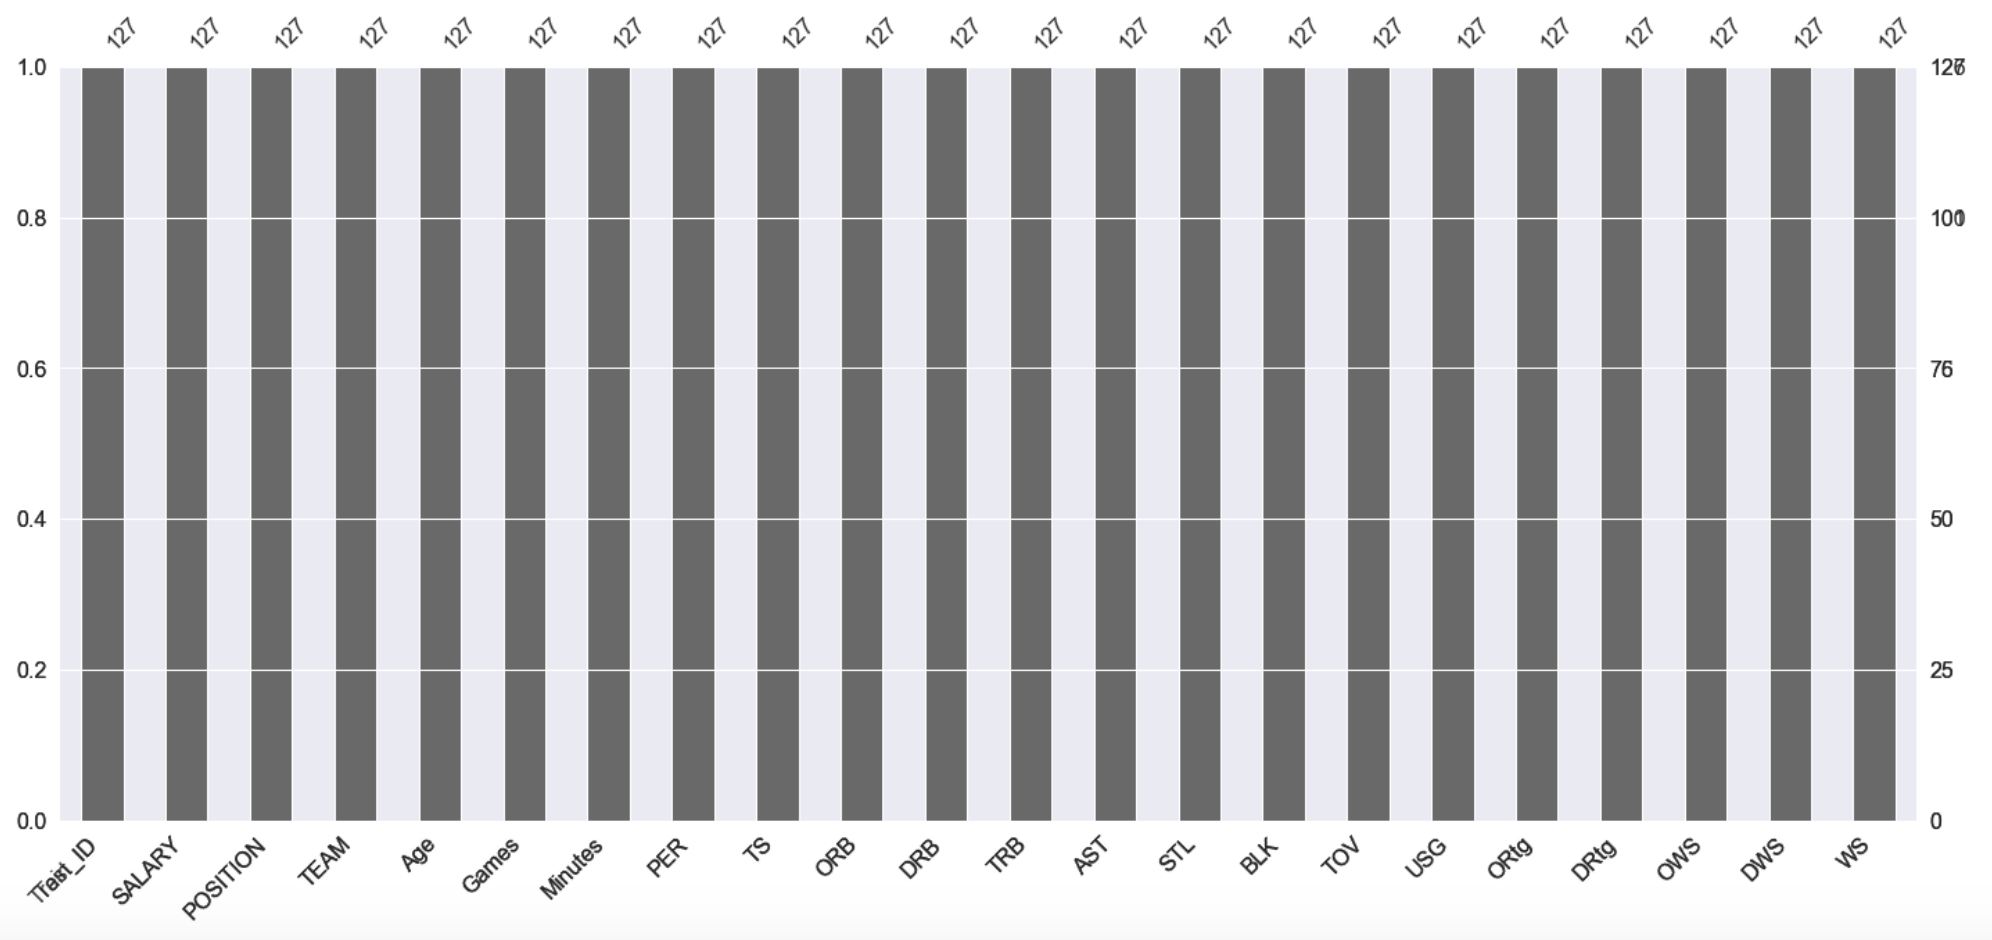
\includegraphics[width=0.9\linewidth, height=5cm]{nbaTrain_miss.png} 
\caption{Missingness barchart of the `NBA train` dataset.}
\label{fig:trainMiss}
\end{subfigure}
\begin{subfigure}{0.55\textwidth}
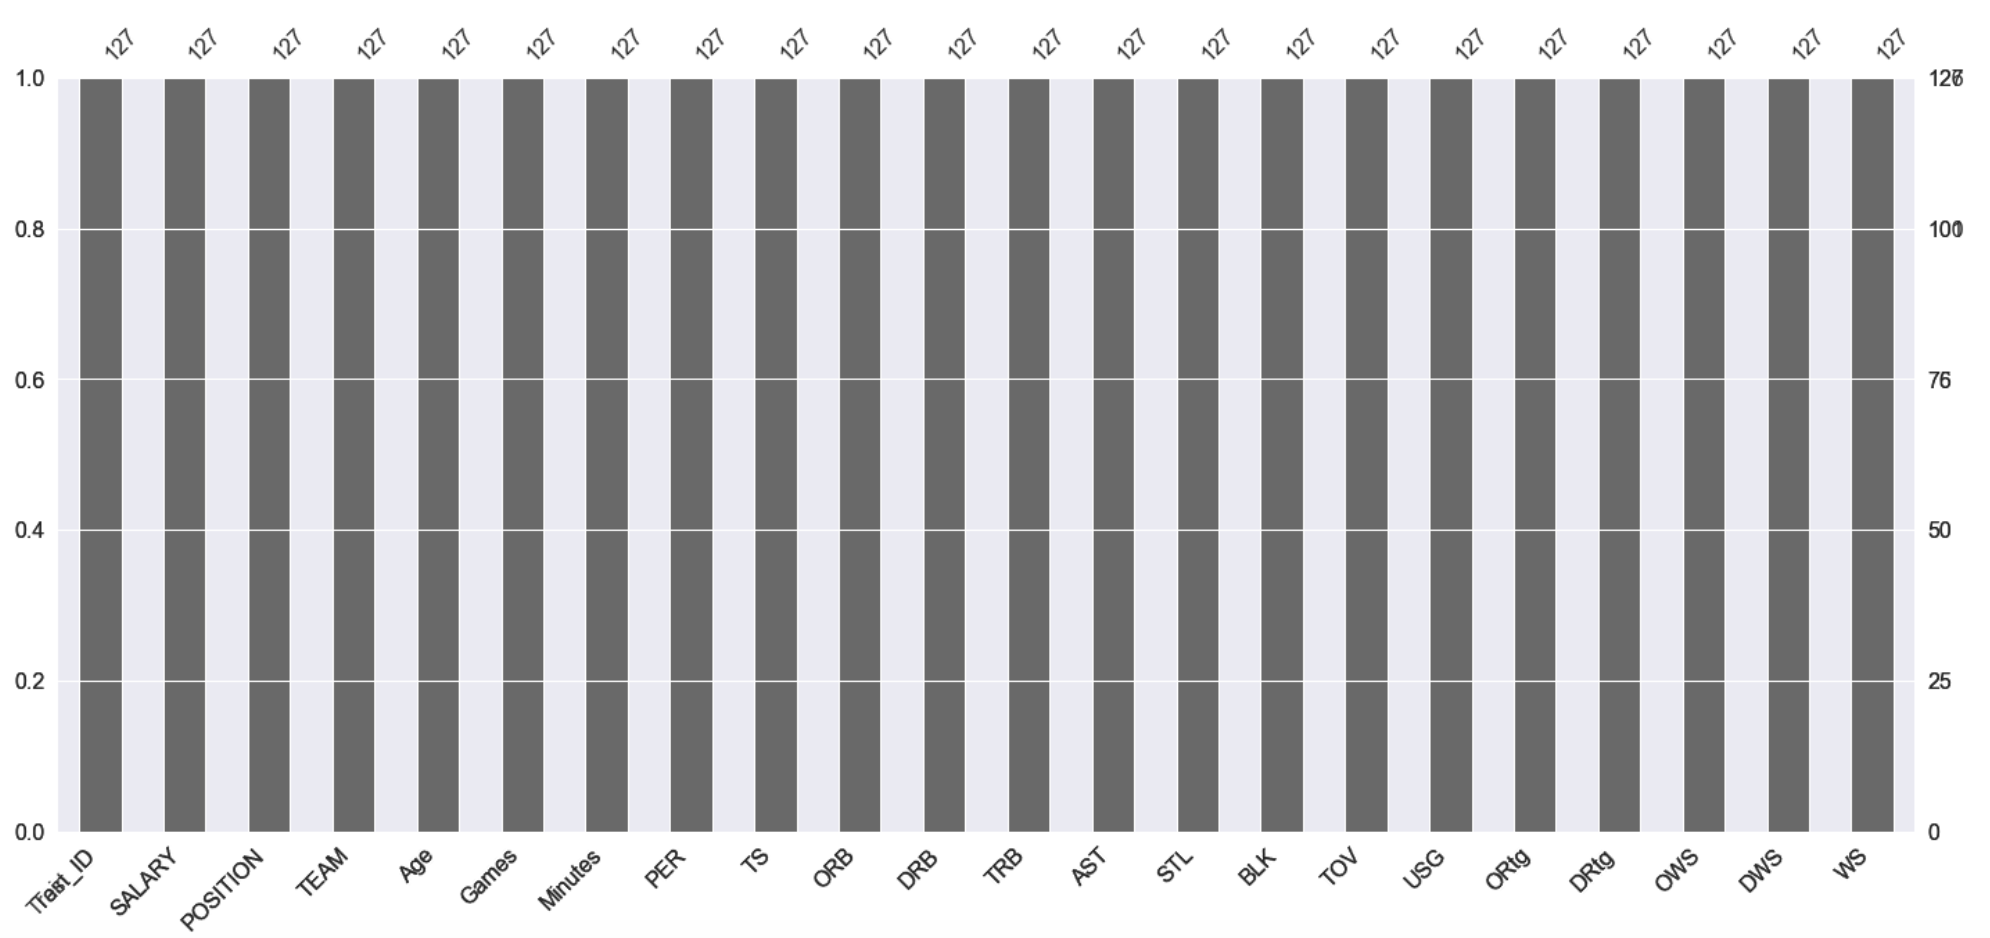
\includegraphics[width=0.9\linewidth, height=5cm]{nbaTest_miss.png}
\caption{Missingness barchart of the `NBA test` dataset.}
\label{fig:testMiss}
\end{subfigure}
\caption{Visualizing the missingness of two datasets used.}
\label{fig:missingness}
\end{figure}

Figure \ref{fig:correlation} illustrate that win share, defensive win
share, offensive win share, number of minutes played and personal
efficiency rate show mediate linear relationships with salary, with win
share having the strongest linear relationship with salary at a
correlation coefficient of 0.68.

\begin{figure}[H]
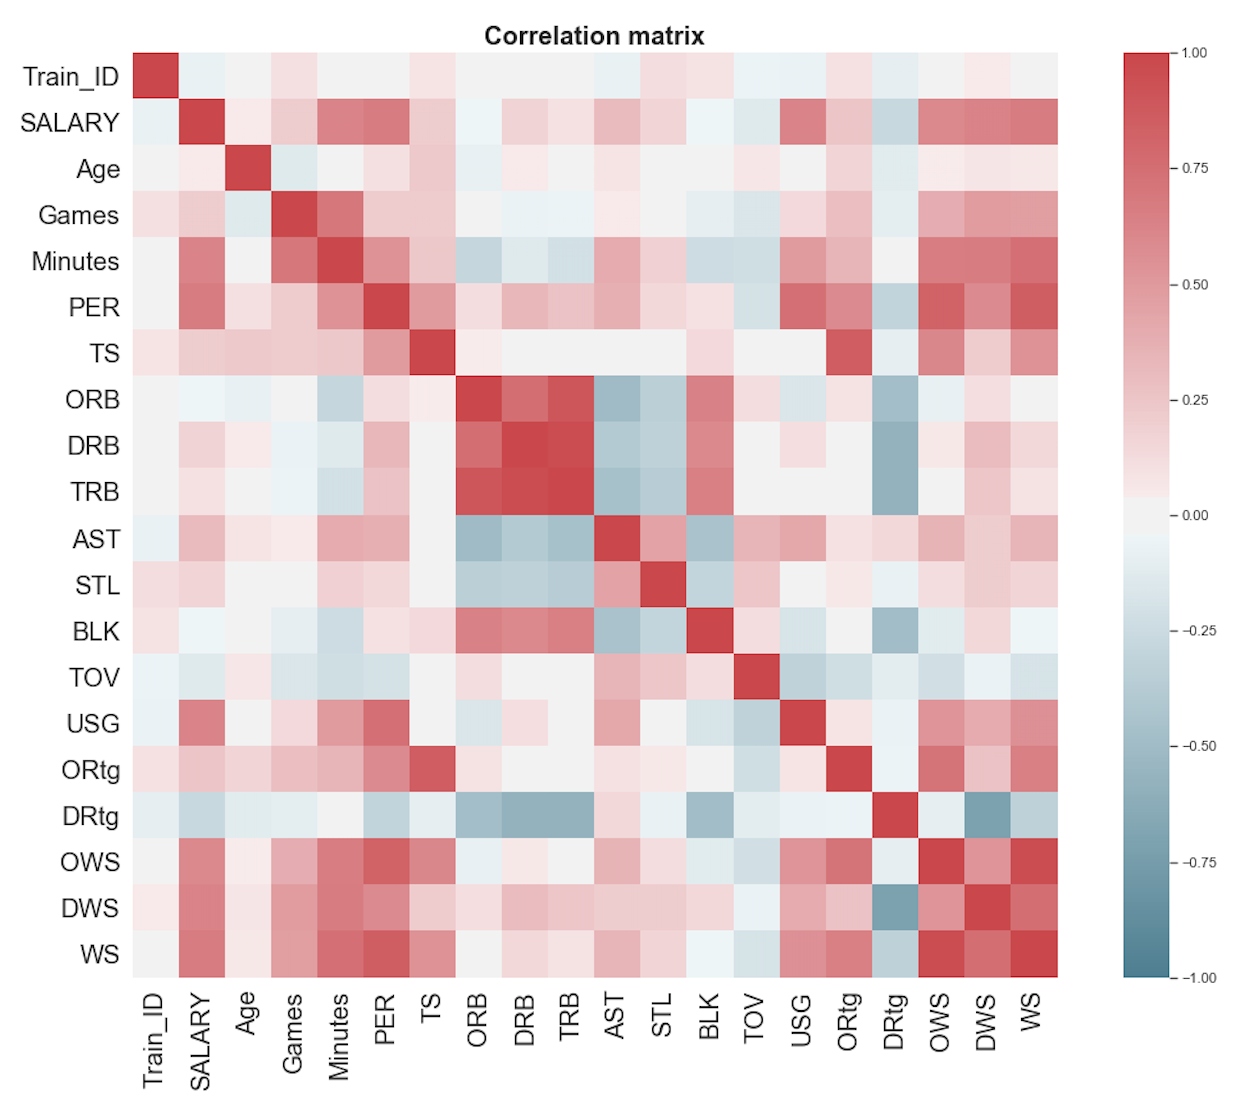
\includegraphics[width=0.8\linewidth]{correlation.png}
\centering
\caption{Correlations between numeric variables based on correlation coefficients.}
\label{fig:correlation}
\end{figure}

The relationships between salary and the six relative variables as well
as the distributation of numeric variables are further visualised by a
scatter plot matrix Figure \ref{fig:scatter}.

\begin{figure}[H]
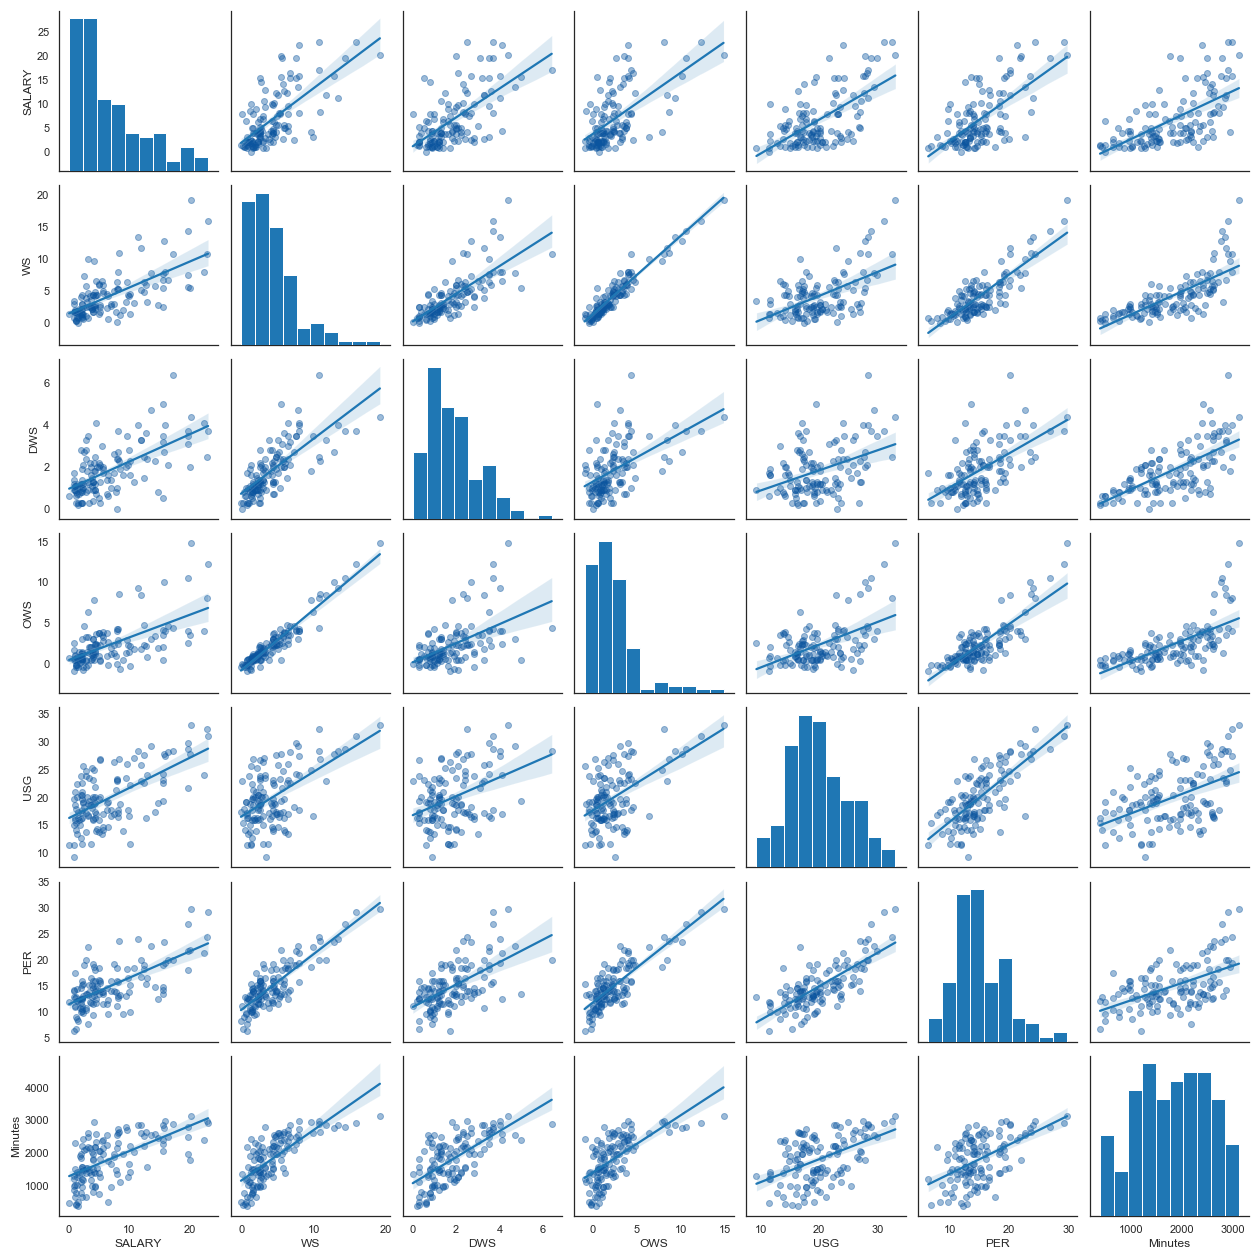
\includegraphics[width=0.8\textwidth]{scatter.png}
\centering
\caption{Caption}
\label{fig:scatter}
\end{figure}

\begin{figure}[H]
\begin{subfigure}{0.55\textwidth}
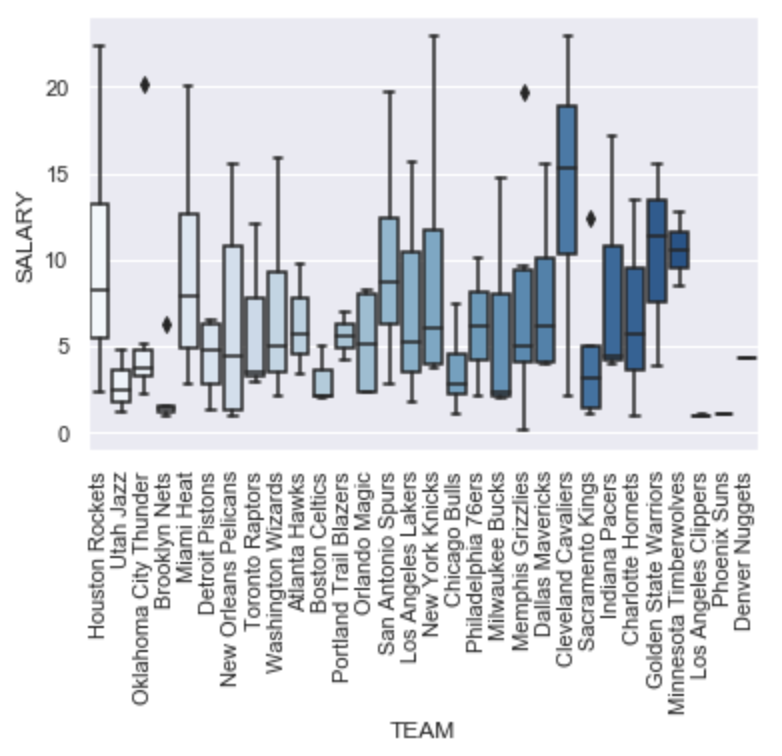
\includegraphics[width=0.9\linewidth, height=5cm]{team_box.png} 
\caption{Salaries for players in different teams.}
\label{fig:subim1}
\end{subfigure}
\begin{subfigure}{0.55\textwidth}
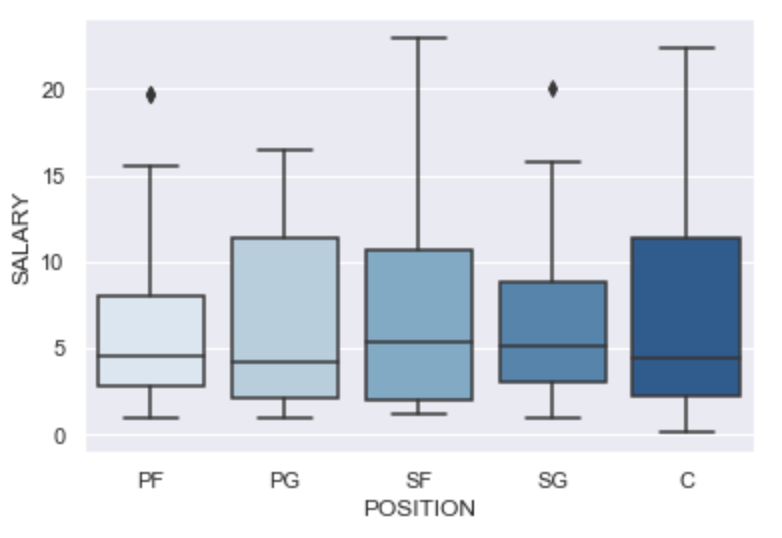
\includegraphics[width=0.9\linewidth, height=5cm]{position_box.png}
\caption{Salaries for players in different positions.}
\label{fig:subim2}
\end{subfigure}
\caption{Box plots of salaries for players in different teams and positions.}
\end{figure}

\hypertarget{feature-engineering}{%
\section{Feature engineering}\label{feature-engineering}}

\hypertarget{methodology-of-the-linear-regression-and-knn-regression-models}{%
\section{Methodology of the linear regression and kNN regression
models}\label{methodology-of-the-linear-regression-and-knn-regression-models}}

\begin{figure}[H]
\begin{subfigure}{0.5\textwidth}
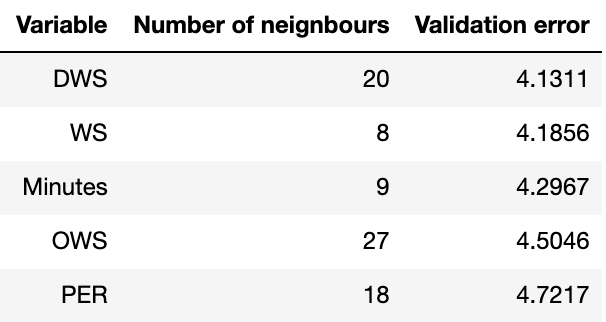
\includegraphics[width=0.9\linewidth, height=5cm]{knn_models.png} 
\caption{Top 5 K nearest neighbor models with the highest validation errors.}
\label{fig:subim1}
\end{subfigure}
\begin{subfigure}{0.5\textwidth}
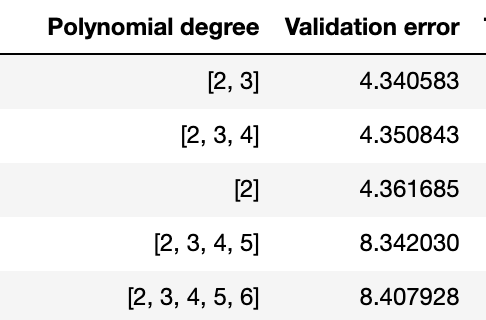
\includegraphics[width=0.9\linewidth, height=5cm]{poly_models.png}
\caption{Top 5 polynomial linear regression models with the highest validation errors.}
\label{fig:subim2}
\end{subfigure}
\caption{Validation errors of 10 models developed.}
\end{figure}

\hypertarget{methodology-of-the-model-that-is-not-covered-in-this-unit}{%
\section{Methodology of the model that is not covered in this
unit}\label{methodology-of-the-model-that-is-not-covered-in-this-unit}}

\hypertarget{test-set-performance}{%
\section{Test set performance}\label{test-set-performance}}

%\showmatmethods


\renewcommand\refname{Analysis and conclusions}
\bibliography{pinp}
\bibliographystyle{jss}



\end{document}

